\section {Measurement Circuitry}
\label{sec:measCirc}
This section describes the schematic design, see Appendix: \ref{app:schematic}, used to meet the goals set out in the \nameref{sec:abstract}. At the time of this writing, this circuit has not been constructed, so what follows will be a theoretical explanation of the circuit's operation. The design builds on the capacitor anodization work done under the ARPA-E contract DE--AR000016 \cite{steve_thesis}.

The purpose of this circuit is to measure the response of a capacitor to various test inputs in order to generate a model (Section: \ref{sec:regression}). This method will allow an analysis of the effect of the DC bias on the output model.

This circuity provides for two main testing modes. In the first mode, a large (up to 500VDC) bias voltage is coupled onto an AC signal via an optocoupler. This voltage is then applied to the \gls{dut} and the resulting current flow is measured through a transimpedance amplifier. The signal is then filtered and its magnitude and phase are measured and digitized. The user has control of the DC bias, AC amplitude, and frequency. These control parameters can be swept to obtain a characterization of the \gls{dut}.

The second test mode provides a means to measure the discharge characteristics of the device. A DC bias is used to charge up the \gls{dut} and then disconnected. The circuity can either connect a discharge capacitor to the \gls{dut} or leave it open in order to measure the discharge current.


\nocite{my_ieeePaper}

\subsection {Power}

The power supply \hyperlink{sch:Power}{circuitry} shows the complete power generation scheme used for the circuit board. 24VDC is fused and then fed through an EMC compliance filter \cite{5VswitchDatasheet}. The initial fuse value is set to roughly twice the current rating of the switching power supplies. Once a practical current draw value is obtained, this value can be decreased. In order to ensure that the three switching regulators meet their rated regulation specifications, output shunt resistors are used to set a minimum load of $10\%$. All of the power supplies were chosen such that their power ratings were at least twice the maximum expected load. The power supply generating $\pm 15V_{ISO}$ is slightly different than the rest, as its output ground is attached to the DC bias voltage instead of signal ground. This purpose of this seen in the optocoupler circuitry described in Section: \ref{sec:opto}.  


\subsection {DC Bias}
\label{sec:dcBias}

The DC bias control \hyperlink{sch:dcBias}{circuitry} controls a Stanford Research Supply SRS-PS350 power supply to generate the bias voltage for the circuit. Some of the models of this supply provide a serial input which can be used to set their output voltage. This scenario is preferred and the communications for it are handled through the RS232 transceiver found on Schematic Page: 3. Other models of this supply only provide an analog input option to control their output voltage. The specifications for this method are shown in Table: \ref{table:srsCtrl_table}. The control signal is generated by using the microcontroller to set the \gls{dac} output over a SPI bus. It is then buffered and clamped to under 1.5V. Since the SRS-PS350 has a gain of 500, this clamps its output to 750VDC. The circuit is only designed to operate at up to 500VDC, but this value is still within the specified ratings of the components in the signal path.

\begin{table}[ht!]
\centering
\begin{tabular}{| l | l | }
\hline
Input Scale      & 0 to +10V for 0 to 5kV                          \\ \hline
Input Impedance  & 1 M$\Omega$                                     \\ \hline
Accuracy         & $\pm 0.2\%$ of full scale                       \\ \hline
Update Rate      & 15 Hz                                           \\ \hline
Output Slew Rate & \textless 0.3s for 0 to full scale (full load)  \\ \hline
\end{tabular}
\caption{SRS-PS350 Analog Control Characteristics \cite{srsManual}\cite{srsCatalog}}
\label{table:srsCtrl_table}
\end{table}


The \gls{dac} has a 2.5V internal reference with a 14 bit resolution, giving the control signal an ideal resolution of $150\mu V$ and the SRS-PS350 an ideal output resolution of $76mV$. The update rate of this device is not important to this application because the \gls{dac} will be set infrequently and only when the system is not actively collecting data.

If different characteristics are needed, the SRS-PS350 can be exchanged for an alternate power supply, but the control logic may not be supported.


\subsection{Optocoupler}
\label{sec:opto}

This section describes the circuitry shown on Schematic Page: 7. It is based upon IXYS's application note AN-107 \cite{locAppNote}, and its purpose is to inject an AC signal ontop of a high DC bias. The optocoupler is configured in what is known as photovoltaic mode \cite{locAppNote}[Sec: 3.3], with both photoreceivers acting as coupled current sources.

In this mode, the front end op-amp's feedback path causes the first photoreceiver to draw current through the first resistor such that both of its terminals stay and ground potential. The phototransmitter's resistor sets a full scale current of 20mA, which is well within the absolute maximum ratings of the device. The second phototransmitter pulls current through the the backend op-amp's feedback resistor with a voltage gain of 2.5.

The output of the optocoupler is referenced to the DC bias voltage from the SRS-PS350 istead of to circuit ground. The limiting isolation specification comes from the $\pm 15V$ supply at 1.5kV, far below the 500V limit imposed by the system. The input sine wave is fed into the magnitude and phase measurement circuitry seen on Schematic Page: 8. The optically coupled sine wave is fed into the DUT as seen on Schematic Page 4.


\subsection{Charging Circuitry}
\label{sec:charging}

The \gls{dut} charging \hyperlink{sch:discharging}{circuitry} is meant to only be used to prepare the \gls{dut} for a test. The current is purposely limited in order to minimize the load on the SRS-PS350. The charging operation functions by enabling the high-current measurement and charging relays, and then slowly ramping the DC bias voltage until the \gls{dut} is fully charged.


\newpage
\section{Discharge Equations}
\label{app:disChargeEqs}
This section lists the discharge equations from Miller's electrochemical capacitor model \cite{electrochem_intro} seen in Figure: \ref{fig:superCap}.

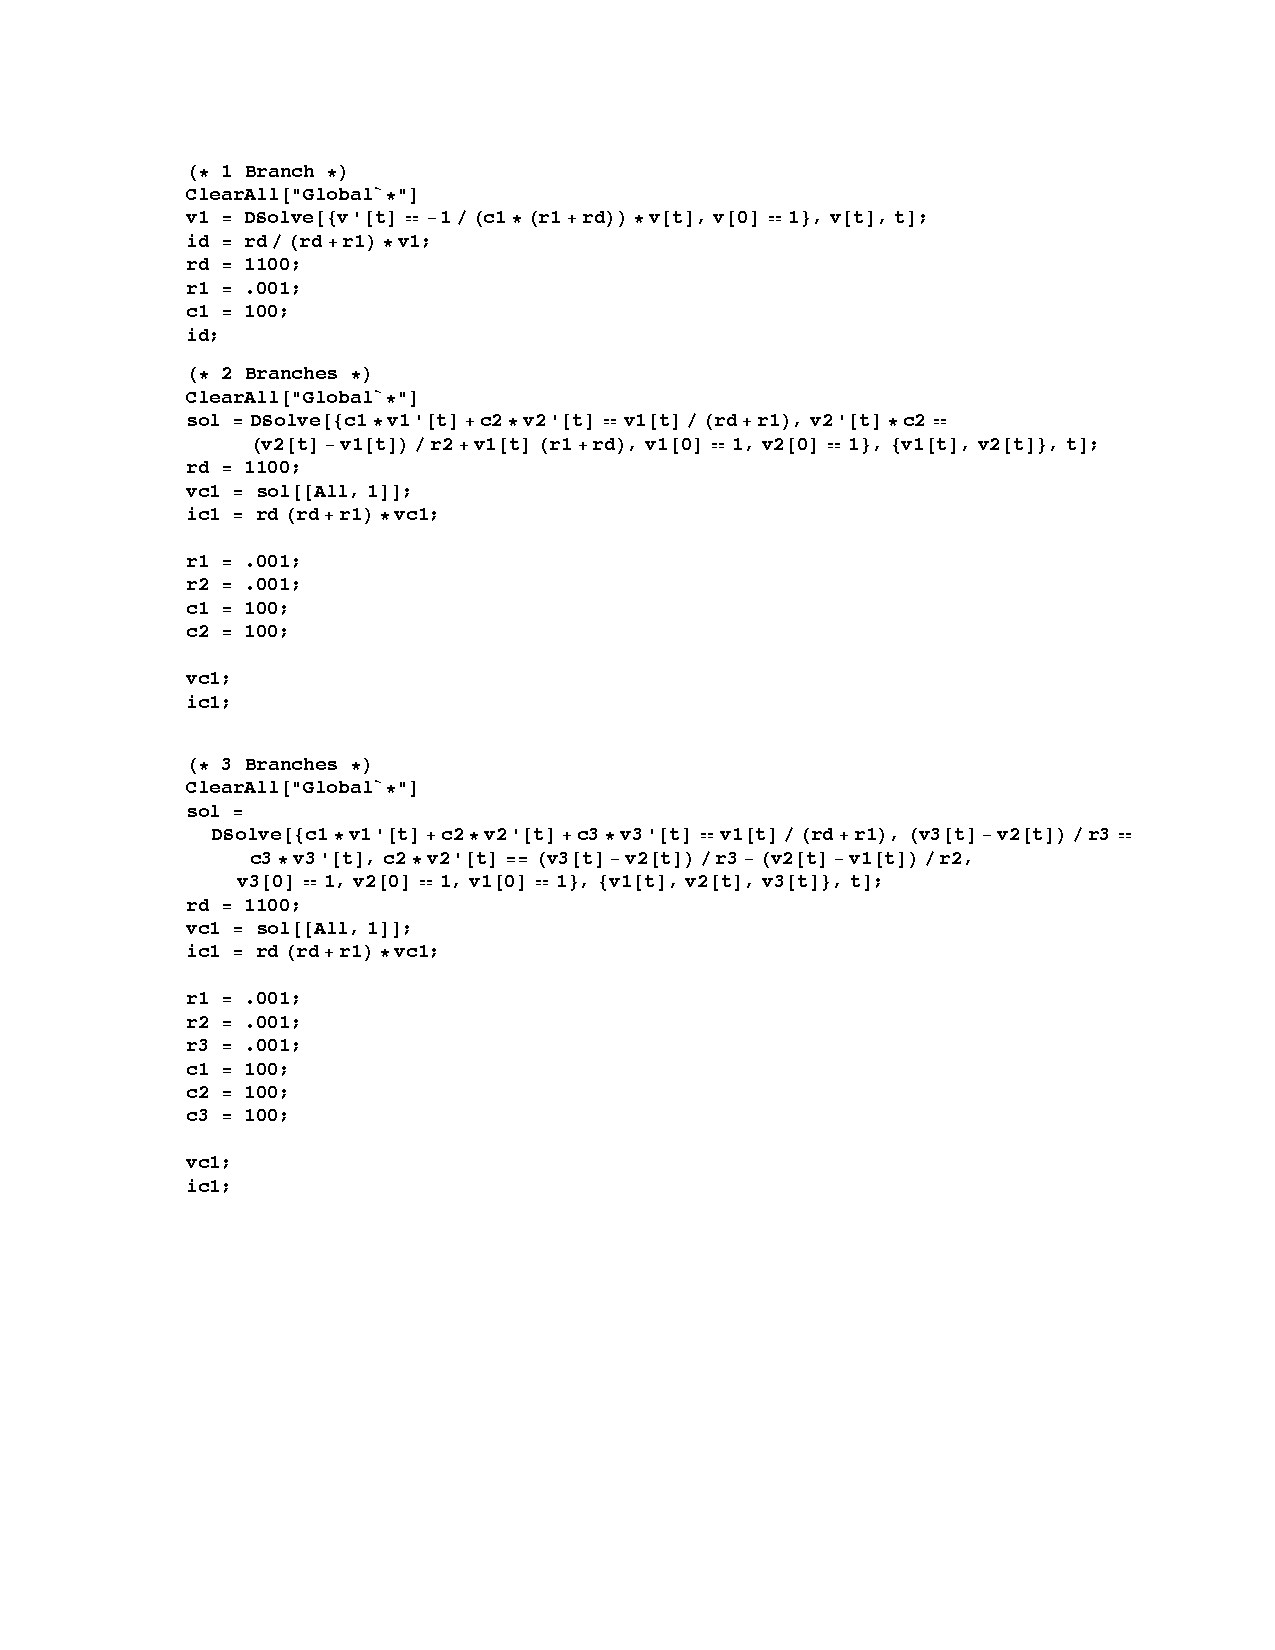
\includepdf[pages=-,offset=1.3in -1.3in,pagecommand={}]{scripts/discharge/discharge.pdf}

\subsection{Current Measurement}

Each of the tests utilize the low-side current measurement circuit. The AC measurement tests provide a known voltage across the DUT and then the current is used to construct the impedance. The discharge tests use the current measurement circuit to capture the current through the DUT over time as its energy drains. 

\subsection{Current Measurement}

Each of the tests utilize the low-side current measurement circuit. The AC measurement tests provide a known voltage across the DUT and then the current is used to construct the impedance. The discharge tests use the current measurement circuit to capture the current through the DUT over time as its energy drains. 

\subsection{Current Measurement}

Each of the tests utilize the low-side current measurement circuit. The AC measurement tests provide a known voltage across the DUT and then the current is used to construct the impedance. The discharge tests use the current measurement circuit to capture the current through the DUT over time as its energy drains. 

\input{tables/imeas}

The current measurement circuit utilizes a transimpedance amplifier designed from the reference circuit in \cite{steve_thesis}. It utilizes 3 switched, feedback stages to measure 9 decades of current (See Table: \ref{imeas_table}). The circuit creates a virtual ground at the negative terminal of the DUT and then uses one of the feedback paths to create a voltage for a digitizer. Using a low-side current measurement circuit is beneficial in this circumstance because it allows low voltage circuitry to condition and measure a signal without needing to see the high DC voltage on the positive terminal of the DUT. The output voltage is calculated by Equation: \eqref{trans}.

\begin{equation}
\label{trans}
Vo = I*R_f
\end{equation}

*Add transistor in increase the Op Amp's current drive capability.
*Change capacitors in feedback loop.
*Add Sallen-key filter to output
*Explain difference in two buffering stages


The output will be buffered and then filtered and digitized dependent of the specific test of interest.



The current measurement circuit utilizes a transimpedance amplifier designed from the reference circuit in \cite{steve_thesis}. It utilizes 3 switched, feedback stages to measure 9 decades of current (See Table: \ref{imeas_table}). The circuit creates a virtual ground at the negative terminal of the DUT and then uses one of the feedback paths to create a voltage for a digitizer. Using a low-side current measurement circuit is beneficial in this circumstance because it allows low voltage circuitry to condition and measure a signal without needing to see the high DC voltage on the positive terminal of the DUT. The output voltage is calculated by Equation: \eqref{trans}.

\begin{equation}
\label{trans}
Vo = I*R_f
\end{equation}

*Add transistor in increase the Op Amp's current drive capability.
*Change capacitors in feedback loop.
*Add Sallen-key filter to output
*Explain difference in two buffering stages


The output will be buffered and then filtered and digitized dependent of the specific test of interest.



The current measurement circuit utilizes a transimpedance amplifier designed from the reference circuit in \cite{steve_thesis}. It utilizes 3 switched, feedback stages to measure 9 decades of current (See Table: \ref{imeas_table}). The circuit creates a virtual ground at the negative terminal of the DUT and then uses one of the feedback paths to create a voltage for a digitizer. Using a low-side current measurement circuit is beneficial in this circumstance because it allows low voltage circuitry to condition and measure a signal without needing to see the high DC voltage on the positive terminal of the DUT. The output voltage is calculated by Equation: \eqref{trans}.

\begin{equation}
\label{trans}
Vo = I*R_f
\end{equation}

*Add transistor in increase the Op Amp's current drive capability.
*Change capacitors in feedback loop.
*Add Sallen-key filter to output
*Explain difference in two buffering stages


The output will be buffered and then filtered and digitized dependent of the specific test of interest.


\subsection{Filtering}
\label{sec:filtering}
\nocite{kirk_skey}

The filtering \hyperlink{sch:filtering}{circuitry} implements two filtering paths which each consist of a 6-pole, low-pass, Sallen-Key filter to condition the signal.

\begin{table}[ht!]
\centering
\begin{tabular}{|l|l|l|l|l|}
\hline
{\bf Filter}         & {\bf Filter Order} & {\bf Gain} & {\bf f\_c} & {\bf Stopband Attenuation} \\ \hline
{\bf Discharging}    & 6                  & 1          & 25kHz      & -65dB                      \\ \hline
{\bf AC Measurement} & 6                  & 1          & 100kHz     & -100dB                     \\ \hline
\end{tabular}
\caption{Sallen-Key Filter Specifications}
\label{table:skey}
\end{table}



\begin{equation}
    \label{equ:sk_fc}
    f_c = \frac{1}{2\pi R_2C_2\sqrt{\frac{R_1C_1}{R_2C_2}}}
    ~\cite{hh}[ch~6.3.2.D~equ~6.5~pg~410]
\end{equation}

\begin{equation}
    \label{equ:sk_q}
    Q = \frac{\sqrt{\frac{R_1C_1}{R_2C_2}}}{1 + \frac{R_1}{C_1}}
    ~\cite{hh}[ch~6.3.2.D~equ~6.6~pg~410]
\end{equation}

A generic, single-stage, low-pass, Sallen-Key filter is shown in Figure: \ref{fig:skey}. The filter is basically a 2-pole, passive, RC filter with the ground of $C_1$ tied to $V_{out}$ through the op-amp's active feedback path. This implementation is a simplified version of the Sallen-Key filter with the gain (listed as K in most explanations) equal to 1. The transition frequency and quality factor can be set according to Equations: \eqref{equ:sk_fc} and \eqref{equ:sk_q} respectively by choosing values for the passives.

\begin{table}[ht!]
\centering
\begin{tabular}{|l|l|l|l|l|}
\hline
{\bf Filter}         & {\bf Filter Order} & {\bf Gain} & {\bf f\_c} & {\bf Stopband Attenuation} \\ \hline
{\bf Discharging}    & 6                  & 1          & 25kHz      & -65dB                      \\ \hline
{\bf AC Measurement} & 6                  & 1          & 100kHz     & -100dB                     \\ \hline
\end{tabular}
\caption{Sallen-Key Filter Specifications}
\label{table:skey}
\end{table}



The filters for this circuit were designed with TI's WEBENCH designer \cite{webench}. Table: \ref{table:skey} shows the specifications for each filter. 
The AC current measurement branch has a cutoff frequency of 100kHz. With the overall measurement frequency range capped at 10kHz, this provides sufficient anti-aliasing for the measurement. The discharge measurement filter has a cutoff of 25kHz. With a $1k\Omega$ resistor and a 1uF \gls{dut} having a time constant of $10\mu s$, this provides a sufficient margin for 100 points per time constant requirement while still filtering out higher frequency components.


\subsection{Magnitude}

This setion describes the magnitude circutry shown on Schematic Page: 7. The circuit measures both the magnitude of the input sine wave and the magnitude of the resultant current waveform through the \gls{dut}. The design for this circuit is based off an Analog Device's app not for the AD8277 \cite{absCircuit}.

The function of this circuit is to perform a full-wave rectification operation on the input signal and then pass the output to be filtered and then sampled. The first difference amplifier is configured as a voltage follower. Since it is only powered from a single rail, it passes the positive half of the waveform and shunts the negative half to ground. The second difference amplifier operates in different modes, based upon the output of the first differential amplifier. During the negative going portions of the waveform, its positive terminal is held at ground, and it operates as a unity gain, inverting amplifier. This rectifies the input signal to the output. During the positive going portions of the waveform, positive input terminal is held at the value of the input terminal. This forces the second difference amplifier to act as a voltage follower. The resultant waveform is a full-wave recified version of the input signal. It is then bypassed with an output capacitor and fed into the \gls{adc} to calculate the value of the rms voltage.


\subsection{Phase}

This setion describes the phase circutry shown on Schematic Page: 7. The circuit measures both the phase of the input sine wave and the phase of the resultant current waveform through the \gls{dut}. It uses two, redundant phase measurement techniques.

The first technique utilizes the AD8302, a \gls{rf} phase detector, in a low frequency configuration as per AN-691 \cite{AD8302_AppNote}. The capacitors on the IC inputs tune the front end high pass filter cutoff to roughly 20Hz. The phase measurement is accomplished internally by a magnitude independent phase multiplier configuration. The output conisists of a 10mV per degree signal that is lowpassed at 2Hz to prevent aliasing. The filtered signal is then fed to the ADC for digitization.

The second technique is added for a low frequency comparison against the \gls{rf} phase detector. The comparator acts as a sine to square wave converter. The default configuration relies on the comparator's internal hysteresis, but provisions for wider thresholds are available if needed. The outputs of the two converters are fed into timer inputs on the microcontroller. The phase is then calculated by the \gls{mcu} by measuring the period of the signals and the time difference between their rising edges.


\subsection{ADC}

This section describes the ADC circuitry found on Schematic Page: 8. It makes use of the AD7656, a 6 channel, 250ksps, 16bit, SAR ADC. It sends the converted values to the microcontroller for further processing and analysis via 3 parallel SPI outputs.


\subsection{Communications}

The communications \hyperlink{sch:com}{circuitry} is used to communicate to off-board processors.

\subsubsection{USB}
The \gls{usb} section is used to communicate with a PC for data logging and post processing. This circuitry centers around a FTDI FT232H serial to \gls{usb} chip. It allows seamless \gls{usb} communication to a PC's COM port with the \gls{mcu} only using a single UART port. This significantly lowers the complexity of the communication bus, as the \gls{mcu} is not responsible for running the \gls{usb} stack.

\subsubsection{RS-232}
The board also has two, bidirectional RS-232 ports. They are able to be used for general purposes, but will most often be used for communicating with a sine-wave generator and the DC Bias supply.



